\documentclass[xcolor=dvipsnames]{beamer}
\usepackage[utf8]{inputenc}
\usepackage{xcolor}
\usepackage{graphicx}
\usepackage{MnSymbol}
\usepackage{stmaryrd}
\usepackage{colortbl}
\usepackage{caption}
\usepackage{comment}
\usepackage[utf8]{inputenc}
\usepackage{pdfpages}
\usepackage{listings}
\usepackage{color}
\usepackage{booktabs}
\usepackage{soul}
\usepackage[normalem]{ulem}
\usepackage{amsfonts}
\usepackage{amsmath}
\usepackage{amsthm}
\usepackage{amssymb}
\usepackage{graphicx}
\usepackage{natbib}
\usepackage[toc]{appendix}
\usepackage{epstopdf}
%\usepackage{subcaption}
\usepackage{caption}
\usepackage{subfig}
\usepackage{ulem}
\usepackage{comment}

\newcommand{\sa}{s^0(\alpha,s^\delta)}
\newcommand{\sd}{s^\delta}
\newcommand{\B}{\mbox{Br}}
\newcommand{\sn}{s^{*}(\alpha)}
\newcommand{\ft}{F^{tacit}}
\newcommand{\fc}{F^{com}}

\usepackage{tcolorbox}
\usepackage{lipsum}


%%%%%%%%%%%%%%%%%%%%%%%%%%%%%%%%%%%%%%%%%%%%%%%%%

\usepackage{pgf}
\usepackage{etex}
\usepackage{tikz,pgfplots}
\usepackage[obeyDraft]{todonotes}

\usetheme{Antibes}
%\usetheme{Madrid}
%\usecolortheme[named=Maroon]{structure}
\usecolortheme{dolphin}
\usefonttheme{professionalfonts}
\useoutertheme{infolines}
\useinnertheme{circles}

\newtheorem*{bem}{Bemerkung}

\usepackage{tikz}


%%%%%%%%%%%%%%%%%%%%%%%%%%%%%%%%%%%%%%%%%%%%%%%%%



%%%%%%%%%%%%%%%%%%%%%%%%%%%%%%%%%%%%%%%%%%%%%%%%%
\usepackage{listings}
\usepackage{color}

\definecolor{dkgreen}{rgb}{0,0.6,0}
\definecolor{gray}{rgb}{0.5,0.5,0.5}
\definecolor{mauve}{rgb}{0.58,0,0.82}

\lstset{frame=tb,
  language=Java,
  aboveskip=2mm,
  belowskip=2mm,
  showstringspaces=false,
  columns=flexible,
  basicstyle={\small\ttfamily},
  numbers=none,
  numberstyle=\tiny\color{gray},
  keywordstyle=\color{blue},
  commentstyle=\color{dkgreen},
  stringstyle=\color{mauve},
  breaklines=true,
  breakatwhitespace=true,
  tabsize=2
}
%%%%%%%%%%%%%%%%%%%%%%%%%%%%%%%%%%%%%%%%%%%%%%%%%


\title[Modes of Signaling]{Modes of Signaling and Managerial Collusion}
\author[Aghadadashli and Legros]{Hamid Aghadadashli\inst{a} and Patrick Legros\inst{b}}
\institute[]{\inst{a} Université libre de Bruxelles (ECARES) \and %
                      \inst{b} Université libre de Bruxelles (ECARES), Northeastern University, and CEPR}
\date[April 25, 2019]{BECCLE, April 25, 2019}

%\graphicspath{{Plots/}}

\begin{document}

\begin{frame}
	\titlepage
\end{frame}

\section{Introduction}

\begin{frame}
\frametitle{Introduction - Communication}
Usually, managers are uninformed about each other's willingness to collude. 

 \begin{figure}[!ht]
     \subfloat[Communication in smoke-filled room]{%
       \includegraphics[width=0.5\textwidth]{Plots/smokedroom.png}
     }
     \hfill
     \subfloat[Market signaling]{%
       \includegraphics[width=0.45\textwidth]{Plots/MarketSignaling.jpg}
     }
     \label{fig:dummy}
   \end{figure}

\end{frame}

\begin{frame}
\frametitle{Introduction - Antitrust Fines}
\begin{itemize}
    \item How do the individual antitrust fines and the distribution of fines affect cartel formation?

    \item[] $\rightarrow$ Individual fines transform the usual cheap talk game into a signaling game;
	
	\begin{itemize}
	    \item[$\Rightarrow$] Collusive outcome under perfect information can be replicated in communication game for a large set of fines;
	    
	    \item[$\Rightarrow$] the fines should not be too small or too large.
	\end{itemize}
	
	\item[] $\rightarrow$ The way fines are distributed between the owners and the managers are crucial for the likelihood of communication.
	
	\item Owners can influence the incentive of the managers:
	
	\item[] $\rightarrow$ owners are also responsible when the bonuses are very high and very low.
\end{itemize}
\end{frame}

\begin{frame}
\frametitle{Introduction - Welfare}
The welfare effect depends on the effectiveness of market signaling.
\begin{itemize}
	\item When communication is necessary for coordination:
	
	\item[] $\rightarrow$ high individual and corporate fines can prevent collusion.
	
	\item When managers can coordinate through market actions:
	
	\item[] $\rightarrow$ high individual and corporate fines may lead to market signaling;
	
	\item[] $\rightarrow$ which can be worse for the consumers.
\end{itemize}
\end{frame}

\section{Model}

\begin{frame}
\frametitle{Model}
	\begin{itemize}
		\item We consider two firms with separation of ownership and managerial control.
		
		\item Managers choose the market actions and exert productive effort $e$ at cost $e^2/2$.
		
		\item Managers can have one of the two types:
		
		\item[] ... \textcolor{red}{$\delta$} - who value future profit flows (with a discount rate $\delta$) and may be \textcolor{red}{open to collusion};
				
		\item[] ... \textcolor{blue}{$0$} - who does not value future profit flows and is \textcolor{blue}{not willing to collude}.		
		
		\item A manager is type $\delta$ with a probability of $\alpha$...
		
		\item[] ... $\alpha$ is independent and identical for both managers.
		\end{itemize}
\end{frame}

\begin{frame}
\frametitle{Model - cont.}
	\begin{itemize}
		\item At time $0$, each owner offers a long term contract to its manager.
		
		\item The managers' utility: $U_i(e_i,s_i) = b_i\cdot e_i \cdot \pi_i(s_i,s_j)-\frac{e_i^2}{2}$.
		
		\item The owers' utility: $\Pi_i=(1-b_i)\cdot e_i \cdot \pi_i(s_i,s_j)$.
		
		\item Timing:
	\end{itemize}

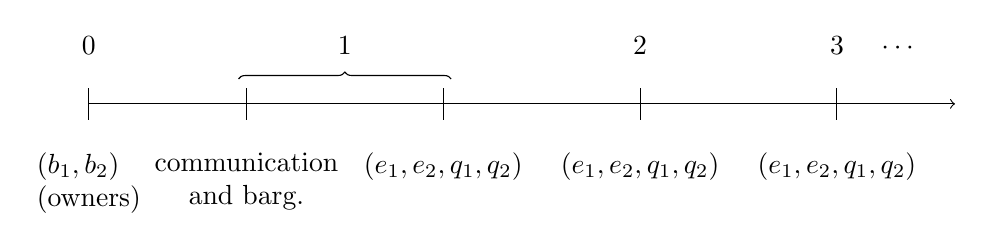
\begin{tikzpicture}

\draw[->] (0,0) -- (11,0);
\draw (0,-.2) -- (0, .2);
\draw (2,-.2) -- (2, .2);
\draw (4.5,-.2) -- (4.5, .2);
\draw (7,-.2) -- (7, .2);
\draw (9.5,-.2) -- (9.5, .2);
\node[align=left, below] at (0,-.5)
{$(b_1,b_2)$\\(owners)};
\node[align=center, below] at (2,-.5)%
{communication \\ and barg.};
\node[align=right, below] at (4.5,-.5)%
{$(e_1,e_2,q_1,q_2)$};
\node[align=right, below] at (7,-.5)%
{$(e_1,e_2,q_1,q_2)$};
\node[align=right, below] at (9.5,-.5)%
{$(e_1,e_2,q_1,q_2)$};
\node[align=left, above] at (0,.5)
{0};
\node[align=center, above] at (3.25,.5)%
{1};
\node[align=right, above] at (7,.5)%
{2};
\node[align=right, above] at (9.5,.5)%
{3};
\node[align=right, above] at (10.3,.5)%
{$\cdots$};
\draw[decoration={brace,raise=9pt},decorate]
  (1.9,0) -- node[above=10pt] {} (4.6,0); 
\end{tikzpicture}		
\begin{itemize}
    \item If managers communicate: both the managers ($f$) and the owners ($F$) expect fines. 
\end{itemize}
		
\end{frame}

\begin{frame}
\frametitle{Separating equilibrium - Managers' problem}
	\begin{itemize}
		\item At time 1
		\item[] $\rightarrow$ type $\delta$ sends message and type $0$ does not;
		
		\item[] $\rightarrow$ if $(com,com)$, type $\delta$ plays $s^M$ and type $0$ plays $BR(s^M)$; 
		
		\item[] $\rightarrow$ otherwise both types play $s^c$ - static competitive equilibrium.
		
		\bigskip
		
		\item At time $t>2$
		
		\item[] $\rightarrow$ if the history is collusive, type $\delta$ plays $s^M$ and type $0$ plays $BR(s^M)$;
		
		\item[] $\rightarrow$ otherwise both types play $s^c$.
		
		\bigskip
		
		\item We look at symmetric equilibria in both managers' and owners' problems.
	\end{itemize}
\end{frame}

\begin{frame}
\frametitle{Separating Equilibrium - IC conditions}
Separation of the types is possible if the following two IC conditions hold:

\begin{equation*}\label{IC-type-delta}
\alpha \frac{1}{1-\delta} \frac{b_i^2 (\pi^M)^2}{2} + (1-\alpha) \frac{1}{1-\delta} \frac{b_i^2 (\pi^c)^2}{2} - f \geq \frac{1}{1-\delta} \frac{b_i^2 (\pi^c)^2}{2}
\end{equation*}

\bigskip

\bigskip

\begin{equation*}\label{IC-type-0}
\frac{b_i^2 (\pi^c)^2}{2}  \geq \alpha \frac{b_i^2 (\pi(Br(s^M),s^M))^2}{2} + (1-\alpha) \frac{b_i^2 (\pi^c)^2}{2} - f.
\end{equation*}
\end{frame}

\begin{frame}
\frametitle{Separating Equilibrium - IC condition for a fixed $F$}
\begin{figure}
\centering
\includegraphics[scale=0.7]{Plots/sep_IC_bonuses.eps}
\caption{IC conditions (red: IC condition for type $0$, blue: IC condition for type $\delta$).}\label{fig:sep_IC_bonuses}
\end{figure}
\end{frame}

\begin{frame}
\frametitle{Separating Equilibrium - Result I}
For a given $b$, there exists $[\underline f(b),\overline f(b)]$ s.t. whenever $f \in [\underline f(b),\overline f(b)]$, there exists an equilibrium strategy of the game with imperfect information and costly communication  that leads to the same outcomes as the games of perfect information.
\end{frame}

\begin{frame}
\frametitle{Separating equilibrium- optimal bonuses}
\begin{figure}[h!]
\centering
\includegraphics[]{Plots/bonuses_diff.eps}
\caption{Bonus levels}\label{fig:bonuses}
\end{figure}
\end{frame}

\begin{frame}
\frametitle{Separating equilibrium}
\begin{figure}[h!]
\centering
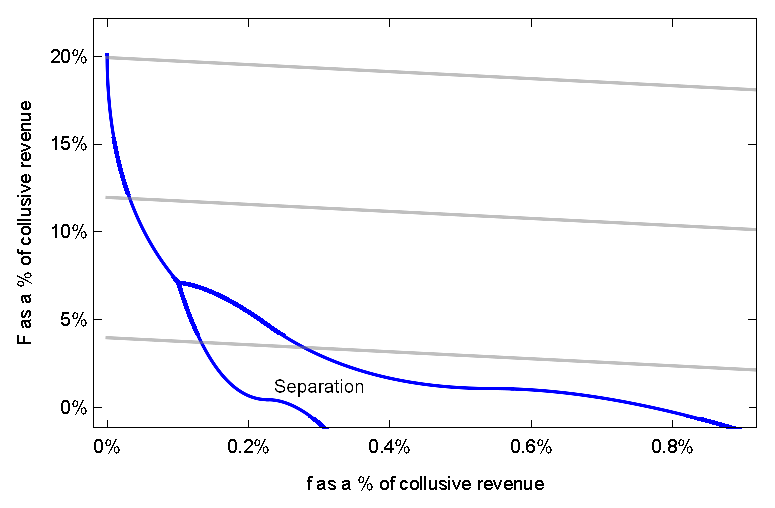
\includegraphics[scale=0.7]{Plots/com_f_F_lines_1_woe.eps}
\caption{Owner-optimal induced communication strategy of the manager given $f,F$.}\label{fig:fines}
\end{figure}
\end{frame}

\begin{frame}
\frametitle{Pooling equilibrium - managers' strategies}
	\begin{itemize}
		\item At time 1
		\item[] $\rightarrow$ both types send message;
		
		\item[] $\rightarrow$ if messages are $(m,m)$, type $\delta$ plays $s^\delta$ and type $0$ plays $BR(s^\delta)$; 
		
		\item[] $\rightarrow$ otherwise both types play $s^c$.
		
		\bigskip
		
		\item At time $t>2$
		
		\item[] $\rightarrow$ if the history is collusive, type $\delta$ plays $s^M$ and type $0$ plays $BR(s^M)$;
		
		\item[] $\rightarrow$ otherwise both types play $s^c$.
	\end{itemize}
\end{frame}

\begin{frame}
\frametitle{Pooling equilibrium - IC conditions}
\begin{figure}[h!]
\centering
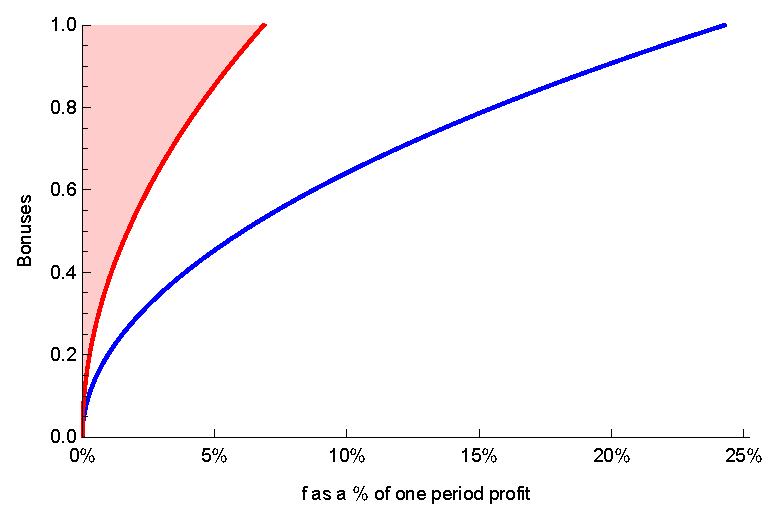
\includegraphics[scale=0.7]{Plots/bonuses_diff_bonus_pool.eps}
\caption{IC conditions (red: IC condition for type $0$, blue: IC condition for type $\delta$).}\label{fig:pool_IC_bonuses}
\end{figure}
\end{frame}

\begin{frame}
\frametitle{Pooling equilibrium - bonuses}
\begin{figure}[h!]
\centering
\includegraphics[scale=0.7]{Plots/bonuses_diff_bonus_pool2.eps}
\caption{Bonus levels in pooling equilibrium.}\label{fig:bonuses_pooling}
\end{figure}
\end{frame}

\begin{frame}
\frametitle{Pooling equilibrium}
\begin{figure}
\centering
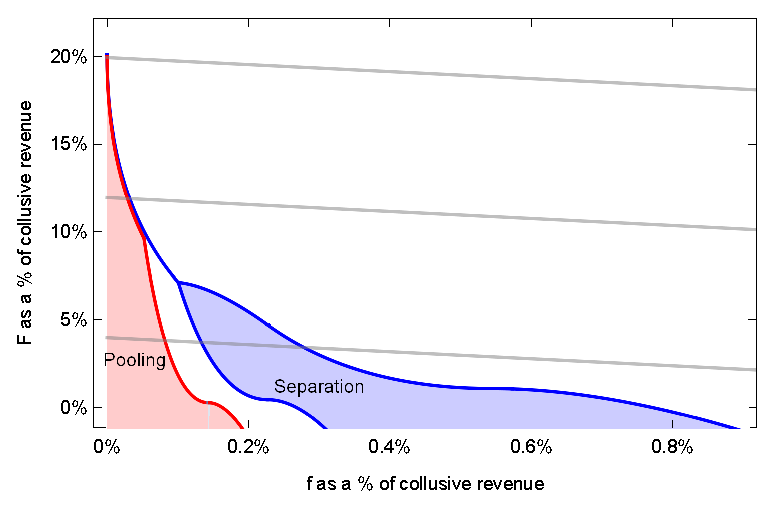
\includegraphics[scale=0.7]{Plots/com_f_F_lines_Sep_pool_woe.eps}
\caption{Separating vs pooling equilibrium.}\label{fig:fines_pool_sep}
\end{figure}
\end{frame}

\begin{frame}
	\frametitle{Value of Communication I}
	If tacit collusion is not possible, collusion can be prevented by high fines $(f,F)$:
	\begin{itemize}
		\item[$\Rightarrow$] higher consumer surplus;
		
		\item[$\Rightarrow$] lower utility for the managers;
		
		\item[$\Rightarrow$] lower profit for the firms.
	\end{itemize}
\end{frame}

\begin{frame}
\frametitle{Market signaling}
\begin{itemize}
\item If tacit collusion is possible, managers can also signal their types by market actions.

\item Belief structure and the strategies of the players will be the same as in pooling equilibrium (after the communication stage).

\item Differences from the pooling equilibrium

\item[] $\rightarrow$ no fines $\Rightarrow$ different IC conditions;

\item[] $\rightarrow$ managers' strategies are independent of the bonus levels $\Rightarrow$ $b_1=b_2=1/2$.
\end{itemize}
\end{frame}

\begin{frame}
\frametitle{Corporate responsibility}
\begin{figure}[!]
\centering
\includegraphics[scale=0.7]{Plots/bonuses_gen.eps}
\caption{Bonuses in communication equilibria.}\label{fig:cs}
\end{figure}
\end{frame}

\begin{frame}
	\frametitle{Value of Communication II}
	If market signaling is possible, high fines $(f,F)$ may lead to market signaling:
	\begin{itemize}
		\item[$\Rightarrow$] market signaling creates inefficiency in the first period and delays coordination;
		
		\item[$\Rightarrow$] consumers and managers may be worse off in market signaling than in communication equilibrium;

		\item[$\Rightarrow$] owners is better off in market signaling than in communication equilibria.
	\end{itemize}
\end{frame}

\begin{frame}%[plain]
\frametitle{}
	\bigskip
	\begin{center}
		{ \textbf{Thank you for your attention!} }
	\end{center}
\end{frame}

%%%%%%%%%%%%%%%%%%%%%%%%%%%%%%%%%%%%%%%%%%%%%%%%%%%
\end{document}
